
\def\>{\rangle}
\def\<{\langle}

%\DeclareMathOperator{\mix}{mix}
%\DeclareMathOperator{\component}{comp}
%\DeclareMathOperator{\cospan}{cospan}
\newcommand\mix{\mathrm{mix}}
\newcommand\component{\mathrm{comp}}
\newcommand\cospan{\mathrm{cospan}}
\newcommand\dist{\mathrm{dist}}
\newcommand\hull{\mathrm{hull}}
\newcommand\support{\mathrm{supp}}

\newcommand\vspan{\mathrm{span}}
\newcommand\cl{\mathrm{cl}}

\def\distinct{\perp}
\def\disjunct{\upmodels}

\newcommand{\ens}[1][e] {\mathsf{#1}} % Ensemble
\newcommand{\Ens}[1][E] {\mathcal{#1}} % Ensemble space

\chapter{Ensemble spaces}

Here we summarize the work in progress for a general theory of states and processes that is applicable to any physical system. The tentative core concept is the ensemble, therefore we want to find definitional requirements for ensembles and then find suitable assumptions to recover the different theories (e.g. classical, quantum and thermodynamics).

 Conceptually, we want to argue that physical theories are, and can only be, about ensembles. At a practical level, most of the time we can only prepare and measure statistical properties as we do not have perfect control over any system. The cases where properties can be prepared with one hundred percent reliability can still be understood as ensembles of identical preparations, though one can argue for an ensemble of external conditions or internal dynamics. At a conceptual level, the goal of physics is to write laws that apply all the time: every time that one prepares a system according to a particular procedure, lets it evolve in particular conditions, he will obtain a particular result. That is, the idea of repeatability of experimental results implicitly assumes that the objects of scientific inquiry are not single instances, but the infinite collections of all reproducible instances.

\section{Ensembles}

TODO: Preamble that argues the justification with physics examples.

\begin{mathSection}
	\begin{axiom}[Axiom of ensembles] 
		The state of a system is represented by an \textbf{ensemble}, which represents all possible preparations of equivalent systems prepared according to the same procedure. The set of all possible ensembles for a particular system is an \textbf{ensemble space}. Formally, an ensemble space is a $T_0$ second countable topological space where each element is called an ensemble.
	\end{axiom}
	
	\begin{justification}
		In physics, ensembles are usually defined as probability distributions over states. This is conceptually problematic. Any actual physical preparation is always associated with some uncertainty. That is, the system will never be replicated exactly. This is true even in quantum mechanics: while we can always prepare a hydrogen atom in the ground state, we can never prepare an atom in the same exact position with the same exact velocity. The ability to prepare ensembles in which the position and the excitation of the atom can be assumed to be uncorrelated is what allows us to concentrate on one of the properties. Therefore, ensembles are the only thing that can actually be prepared in practice. Pure states, then, should not be taken as primitive notions but should be understood as an idealized ensemble. 
		
		From a more conceptual level, reproducibility is baked into the requirement of experimental verifiability. A physical law, then, must be understood as describing a relationship that always exist whenever the same set of circumstances is replicated. Given that we need to always be able to replicate those circumstances ``one more time'', the relationship is about countably infinite similar preparations: an ensemble. Therefore, to the extent that physics is about reproducible experimental results, the basic description of a system is in terms of ensembles. This justifies the use of ensembles as the fundamental object to describe the state of a system.\footnote{Note that reproducibility also already implies that all properties that characterize an ensemble must be relative to the procedure. If the properties depended, for example, on absolute space or absolute time, then different practitioners would not be able to prepare the same ensemble.}
		
		Ensembles are experimentally defined objects, and therefore they are possibilities of an experimental domain. Therefore an ensemble space is a $T_0$ second countable topological space where each element is an ensemble and the topology is induced by the verifiable statements.
	\end{justification}
\end{mathSection}

A general theory of ensembles will need to be able to recover classical and quantum spaces under appropriate physically meaningful assumptions. Here we review these cases and give the appropriate mathematical definitions, highlighting potential issues, as these serve as models and examples for a general theory.

There are two aspects that are common to all cases and will be the target of generalization: statistical mixing (captured by a convex structure) and entropy (captured by a strictly concave function). Note: all $\log$s are assumed in base 2.

\subsection{Discrete classical theory}

\begin{defn}
	The ensemble space of a \textbf{discrete classical theory} is a simplex with the standard convex structure and the Shannon entropy. The simplex can have finitely or countably many vertices.
	
	That is, a discrete classical ensemble space is a set $\Ens$ containing $n$ points $\{s_i\}^n_{i=1}$ and for which every element $\ens \in \Ens$ is characterized by a unique convex combination $\ens = \sum_i p_i s_i$ such that $\sum_i p_i = 1$. The space is closed under convex combinations of finitely many elements. The entropy is given by $S(\ens) = - \sum_i p_i \log p_i$.
\end{defn}

\begin{remark}
	The correct closure under convex combinations of countably many elements is not clear.
\end{remark}

\subsubsection{Finite case}

The space of classical distributions over a discrete space corresponds to a simplex (\url{https://en.wikipedia.org/wiki/Simplex}). In the finite case, the pure states $\mathcal{S} = \{s_i\}_{i=1}^{n} \subset \Ens$ are finitely many and each ensemble $\ens = \sum p_i s_i$ is uniquely identified by a decomposition of pure states. Effectively, each ensemble is a probability distribution over the pure states. Mathematically, each point of the space is a convex combination of the vertices. The simplex has a center point, which corresponds to the maximally mixed state, a uniform distribution over all pure states. 

The entropy is given by the Shannon entropy $-\sum_i p_i \log p_i$. This means that the entropy of each pure state is zero and the entropy of the maximally mixed state is $\log n$ where $n$ is the number of pure states. The entropy increases as we go from pure states to the maximally mixed state. The level sets (i.e. the fibers) of the entropy form a series of concentric ``shells''.

The fact that all pure states have the same entropy is an additional hypothesis that cannot work in general. To see this, consider the case where the state is defined by the number of molecules for two substances. This space is the product of two independent variables $n_a$ and $n_b$. If we have a uniform distribution over $N_a$ cases of $n_a$ and $N_b$ cases of $n_b$, the total number of cases is $N_a N_b$. Therefore the entropy of the joint state is the sum of the entropy of the marginals. However, if we pair $n_a$ with the total number of molecules $n_{(a+b)}$ we have a problem. The issue is that variable $n_{(a+b)}$ corresponds to a variable number of joint cases. Therefore the case where the ensemble space is a simplex but the entropy is not the Shannon entropy (e.g. is the Shannon entropy plus the contributions of entropy from each vertex) is a physically meaningful case that should be possible in the general theory.

\subsubsection{Countable case}

The countable case is not well-defined mathematically.

The obvious extension is to include all series $\{p_i\} \in [0,1]$ that converge to one. That is, the space of all probability measures over a countable discrete space. Since we cannot create a uniform distribution over infinitely many cases, there is no center point. Effectively, there is a ``hole'' in the middle. More precisely, the space is not topologically closed in the sense it does not contain all the limit points.

[TODO] It may be useful to characterize this ``hole'' and the limit points. There should be at least one limit point for each series $\{p_i\}$ that converges to a finite $p < 1$. Intuitively, we can keep that part of the distribution constant while we spread the rest uniformly to all cases. Each should reach a different limit point.

However, the space of all probability measures is too large. Note that the entropy is not finite for all convergent $p_i$ (i.e. infinite convex combinations). For details, see \url{https://arxiv.org/pdf/1212.5630.pdf}. Given that we want the entropy to exist and be finite for all ensembles, this generalization (like in \url{https://ncatlab.org/nlab/show/superconvex+space} ) does not seem physically warranted.

Also note that expectation values are not guaranteed to be finite either, and requiring a particular observable to be finite further restricts the space. This restriction may be desirable for another reason: a discrete ensemble space has no notion of the ordering of the pure states. Physically, this would mean that the states with 1, 100, or 1 trillion particles are ``equally distant'' (i.e. all infinite permutations are allowed). Requiring the expectation of the number of particles to be finite (e.g. $\sum_i N(i) p_i < \infty$) should effectively encode the infinite ordering in the rate of convergence of the probability distributions (i.e. not all infinite permutations would be allowed).

\subsubsection{No uncountable case}

The uncountably infinite case is not physically relevant (i.e. no second countable discrete topology, cases are not experimentally decidable). Also note that any set of real numbers whose sum is finite can have only countably many non-zero elements. To understand why, note that there can only be finitely many terms above any particular positive value if their sum is to remain finite. Effectively, the uncountable case would be stitching together infinitely many countable cases.

\subsection{Continuous classical theory}

\begin{defn}
	The ensemble space of a \textbf{continuous classical theory} is the convex space given by the probability distributions (i.e. probability measures) over phase space (i.e. a symplectic manifold) that allow a continuous probability density (i.e. the Radon-Nikodym derivative exists - the probability measures are absolutely continuous with respect to the Liouville measure - and is continuous). Formally, let $(X, \omega)$ be a symplectic manifold. The ensemble space is given by $\Ens = \{ \rho \in C(X) \, | \, \int_X \rho d\mu = 1 \} $. The entropy is given by the Shannon/Gibbs entropy calculated using the probability density (i.e. the Radon-Nikodym derivative between the probability measure and the Liouville measure). That is, $S(\rho) = - \int_X \rho \log \rho d\mu$.
\end{defn}

In the continuous case, the space of ensembles is the space of continuous integrable functions over a symplectic manifold (e.g.  over phase space) that integrate to one. That is, if $X$ is a symplectic manifold, then $\Ens = \{ \rho \in C(X) \, | \, \int_X \rho(x) d\mu = 1 \} $ where $\mu=\int \omega^n$ is the Liouville measure. The space does not include the pure states, as they correspond to delta distributions $\mathcal{S} = \{\delta_x\}_{x \in X}$: they are limit points. In some sense, a distribution can be understood as a convex integral of pure states: $\rho(x) = \int_X \rho(y) \delta_x(y) d\mu$. Even in this case, each ensemble can be understood as a unique probability distribution (density in this case) over all pure states. The symplectic nature of the manifold is required to assign a frame invariant density to states and a frame invariant notion of independence between DOFs, as we saw in the classical mechanics section of reverse physics.

The fact that pure states are not part of the space, but limits, means we need a more sophisticated definition of pure states than simply the extreme points of the convex space of ensembles.

The entropy is given by $- \int \rho \log \rho d\mu$ where $\mu$ is the Liouville measure and $\rho$ is the probability density over canonical coordinates. If a different measure is used, or if the coordinates are not canonical, the formula gives the wrong result.

Similarly to the infinite discrete case, the entropy can be infinite and expectation values can be infinite. The added complication is the frame invariance: it would not make sense to have the expectation for position in one frame to be finite while infinite in another. Requiring all functions of position/momentum to have finite expectation restricts the distributions to those with finite support. Requiring all polynomial functions of position/momentum to have finite expectation restricts the distributions to those that decay faster than any polynomial.

Unlike the discrete classical case, subspaces and dimensionality of subspaces cannot be defined without the entropy. The issue is that we need a measure on the set of pure states, and the convex structure cannot provide it. The entropy, however, does as the supremum of the entropy for all distributions with support $U$ is $\log \mu(U)$. As we will see, the entropy can be used to both identify subspaces and recover the Liouville measure.

Note that we exclude discontinuous distributions as starting from the space of discontinuous distributions does not allow one to recover the topology of the base space. Suppose, in fact, to have the space of all distributions over the real line that integrate to one. Now imagine switching the interval $[0, 1)$ with the interval $[1, 2)$. This is an isomorphism on the space of discontinuous distributions. Therefore given the space of distributions, we cannot recover the topology of the real line. Now take the space of continuous functions that integrate to one. Take those with support $[0,1) \cup [2,3)$. This is the set of convex combinations of the distributions with support $[0,1)$ and $[2,3)$ precisely because the sets are not contiguous and the distributions will have to go to zero at the boundary. However, the distributions with support $[0,2)$ are not just the convex combinations of those with support $[0,1)$ and $[1,2)$ because this will include the continuous functions that have a non-zero value at $1$.

[TODO] It may be interesting to study the shell of zero entropy states. For example, it should not be path connected: all uniform distributions with support of the same finite size (in terms of the Liouville measure) will have the same entropy. The region, however, need not be contiguous. Since we cannot continuously transform a single region into two disjoint regions, there will be different distributions at zero entropy that cannot be transformed continuously.


\subsection{Quantum theory}

\begin{defn}
	The ensemble space of a \textbf{quantum theory} is modeled by the convex space given by the density operators (i.e. positive semi-definite self-adjoint operators with trace one) of a Hilbert space equipped with the von Neumann entropy.
	
	That is, given a Hilbert space $\mathcal{H}$, the ensemble space is the space of positive semi-definite self-adjoint operators with trace one $M(\mathcal{H})$. The space of pure states is given by the projective space $P(\mathcal{H})$. The entropy of an ensemble $\rho \in M(\mathcal{H})$ is given by the von Neumann entropy $S(\rho) = -\tr(\rho \log \rho)$.
\end{defn}

\subsubsection{Finite dimensional case}

The simplest non-trivial case is the qubit, for which the Bloch ball is the space of ensembles $M(\mathcal{H})$. The interior of the Bloch ball corresponds to mixtures  while the surface corresponds to the pure states $\mathcal{S} = P(\mathcal{H}) = \{ |\psi\> \<\psi| \}_{\psi \in \mathcal{H}}$. In quantum ensemble spaces there is no unique decomposition. Note that the space is exactly characterized by knowing which different mixtures provide the same ensemble.

The multiple decompositions make the ensemble space behave in a way that is a hybrid between the classical discrete and continuous. Pure states are properly a part of the ensemble space, as in the discrete case, and we can describe each mixture in terms of finitely many pure states. However, the pure states are a continuum, therefore we can also define probability densities over the space, convex integrals. For example, for a single qubit, the maximally mixed state (the center of the ball) can be equally described as the equal mixture of two opposite states (e.g. spin up and spin down, or spin left and spin right). However, it can also be described as the equal mixture of the whole sphere.

Note that complex projective spaces are symplectic, which is what allows one to define frame invariant densities. The goal is to have one argument applied to the generic definition as to why the space of pure states must be symplectic. Also note that the two dimensional sphere is the only symplectic sphere. By homogeneity, we should be able to argue that the space is symmetric around the maximally mixed state, and is therefore a sphere. The symplectic requirement would select dimension two. Note that real and quaternionic spaces would be excluded by this argument.

The von Neumann entropy for the maximally mixed state is $\log n$ where $n$ is the dimensionality of the Hilbert space. Again we see that the maximum entropy gives us a measure of the size of the space. Note that, to calculate the von Neumann entropy, we are diagonalizing the density matrix $\rho$. This means finding a set of orthogonal pure states $s_i$ such that $\rho = \sum p_i s_i$ is a convex combination. Note that the convex hull of a set of $n$ orthogonal pure states is an $n$-dimensional simplex whose center is the maximally mixed state. Therefore, we are looking for a simplex that contains $\rho$ and the maximally mixed state. In the two dimensional case, $\rho$ is an interior point of the Bloch ball. Take the line that connects $\rho$ to the center. The two points of the sphere are the extreme points for the decomposition. The distance from the points will be proportional to the probability. Because of this property, the von Neumann entropy is the smallest Shannon entropy between all possible decompositions.


\subsection{Countably infinite dimensional case}

The countable infinite dimensional case presents similar problems as the classical case, and adds others. As in the classical infinite cases, the maximally mixed state (i.e. uniform distribution) is not in the convex space and the entropy is not finite for all infinite convex combinations. As in the classical continuous case, there is the issue of finite expectation of position/momentum in all frames. The problem is compounded by the fact that one cannot require finite expectation for all functions of position and momentum: finite support in position automatically implies infinite support on momentum, since the distribution in momentum is the Fourier transform of that in position.

The Hilbert space for a discrete variable with infinite range (e.g. number of particles) and a continuous variable (e.g. position/momentum) is the same. The first is defined as the space of square convergent complex sequences $l^2$ while the second is the space of square integrable complex functions $L^2$. Given that $L^2$ allows a countable basis, the two are isomorphic. This also means that all spaces with finitely many degrees of freedom are also isomorphic. This makes the problem of infinite expectations even more problematic.

Note that Schwartz spaces have finite expectation for all polynomial functions of position and momentum. Given that infinite permutations can change the rate of convergence, the Schwartz space has an idea of what is further away from the origin, unlike Hilbert spaces. [TODO] It is not yet clear to us whether the Schwartz space for one DOF is the same as the one for two DOFs.

\section{Mixtures and convex spaces}



\begin{defn}
	Given a real number $p \in [0,1]$, its complement is defined as $\bar{p} = 1-p$.
\end{defn}

\begin{axiom}[Axiom of mixture]
	An ensemble space $\Ens$ is equipped with an operation $+ : [0, 1] \times \Ens \times \Ens \to \Ens$ called \textbf{mixing}, noted with the infix notation $p \ens_1 + \bar{p} \ens_2$, with the following properties:
	\begin{itemize}
		\item \textbf{Continuity}: $p \ens_1 + \bar{p} \ens_2$ is continuous in all its arguments (i.e. $p$, $\ens_1$ and $\ens_2$)
		\item \textbf{Identity}: $1 \ens_1 + 0 \ens_2 = \ens_1$
		\item \textbf{Idempotence}:  $p \ens_1 + \bar{p} \ens_1 = \ens_1$ for all $p \in [0,1]$
		\item \textbf{Commutativity}: $p \ens_1 + \bar{p} \ens_2 = \bar{p} \ens_2 + p \ens_1$ for all $p \in [0,1]$
		\item \textbf{Associativity}: $p_1 \ens_1 + \bar{p_1}\left(\overline{\left(\frac{p_3}{\bar{p_1}}\right)}\ens_2 + \frac{p_3}{\bar{p_1}}\ens_3\right) =  \bar{p_3}\left(\frac{p_1}{\bar{p_3}} \ens_1 +  \overline{\left(\frac{p_1}{\bar{p_3}}\right)}\ens_2\right) + p_3 \ens_3$ for all $p_1, p_3 \in [0,1]$
	\end{itemize}
\end{axiom}

\begin{justification}
	This axiom captures the ability to create a mixture merely by selecting between the output of different processes.
	
	Given that mixing represents an experimental relationship, and all experimental relationships must be continuous in the natural topology, mixing must be a continuous function. Note that $p$ is a continuous quantity, and therefore the natural topology is the one of the reals.

	Let $\ens_1$ and $\ens_2$ be the ensembles that represent the output of two different processes $P_1$ and $P_2$. Let a selector $S_p$ be a process that outputs two symbols, the first with probability $p$ and the second with probability $\bar{p}$. Then we can create another process $P$ that, depending on the selector, outputs either the output of $P_1$ or $P_2$. Therefore we are justified in assuming the mixing operation among ensembles.

	If $p=1$, the output of $P$ will always be the output of $P_1$. This justifies the identity. If $P_1$ and $P_2$ are the same process, then, again, the output of $P$ will always be the output of $P_1$. This justifies the idempotence. As long as the same probability is matched to the same output, the process $P$ is identical. This justifies commutativity. If we are mixing three processes $P_1$, $P_2$ and $P_3$, as long as the final probabilities are the same, it does not matter if we mix $P_1$ and $P_2$ first or $P_2$ and $P_3$. This justifies associativity.
\end{justification}

\begin{remark}
	Given symmetry and associativity, we can write $p_1 \ens_1 + p_2 \ens_2 + p_3 \ens_3$ where $p_2 = \bar{p_1}\overline{\left(\frac{p_3}{\bar{p_1}}\right)} = \bar{p_3}\overline{\left(\frac{p_1}{\bar{p_3}}\right)} = 1 - p_1 - p_3 = \overline{\left(p_1 + p_3\right)}$. We can also extend to mixtures of finitely many elements $\sum p_i \ens_i$ where $\sum_i p_i = 1$.
\end{remark}

\begin{coro}
	An ensemble space is a convex space.
\end{coro}

\begin{remark}
	Basic definitions for convex spaces are taken from \url{https://ncatlab.org/nlab/show/convex+space} and \url{https://arxiv.org/abs/0903.5522}. The notation and terminology will be slightly different to better map to physics ideas. 
\end{remark}


\begin{defn}
	Let $\Ens$ be an ensemble space. Let $\ens[\rho] = \sum_i p_i \ens_i$ where $\ens[\rho], \{\ens_i\} \in \Ens$ and $p_i \in (0,1]$ such that $\sum p_i = 1$. We say that $\ens[\rho]$ is a \textbf{mixture} of $\{\ens_i\}$ and each $\ens_i$ is a \textbf{component} of $\ens[\rho]$.
\end{defn}

\begin{remark}
	In terms of the convex space, all the mixtures between two elements corresponds to the segment between them; all the mixtures between three elements correspond to the triangle formed by the three elements and so on. An element $\ens_1$ is a component of a different element $\ens_2$ if the segment can be continued on the side of $\ens_2$. Note that two elements can be a component of each other. If two elements are not a component of each other, then they are the extreme points of the line that connect the two.
\end{remark}

\begin{defn}
	Let $\Ens$ be an ensemble space and $\ens_1, \ens_2 \in \Ens$. We say that they \textbf{have a common component} if we can find $\ens_3 \in \Ens$ such that $\ens_1 = p_1 \ens_3 + \bar{p_1} \ens_4$ and $\ens_2 = p_2 \ens_3 + \bar{p_2} \ens_5$ for some $\ens_4, \ens_5 \in \Ens$ and $p_1, p_2 \in (0,1)$. They are \textbf{distinct}, noted $\ens_1 \distinct \ens_2$, otherwise.
\end{defn}

\begin{remark}
	In terms of convex spaces, two distinct ensembles are always the extreme points of the line that connects them. Additionally, for any other ensemble $\ens$, one of the two ensembles must be the extreme point of the line that connects it to $\ens$.
\end{remark}

\begin{coro}
	The previous definitions obey the following:
	\begin{enumerate}
		\item every ensemble has a common component with itself, therefore every ensemble is not distinct from itself
		\item distinctness is a irreflexive symmetric relation
		\item if $\ens_1$ is a component of $\ens_2$, then $\ens_1$ and $\ens_2$ have a common component
	\end{enumerate}
\end{coro}

\begin{proof}
	1. Since by idempotence $\ens = p \ens + \bar{p} \ens$ for any $p$, we can satisfy the definition by setting $\ens_1 = \ens_2 = \ens_3 = \ens_4 = \ens_5 = \ens$. Therefore every ensemble has a common component with itself and every ensemble is not distinct from itself.
	
	2. The previous property shows that distinctness is irreflexive. The definition of common component is symmetric and therefore so is distinctness.
	
	3. By idempotence, we can write $\ens_1 = p_1 \ens_1 + \bar{p_1} \ens_1$ for some $p_1 \in (0,1)$. Since $\ens_1$ is a component of $\ens_2$, we can write $\ens_2 = p_2 \ens_1 + \bar{p_2} \ens_3$ for some $p_2 \in (0, 1)$ and $\ens_3 \in \Ens$. Therefore $\ens_1$ and $\ens_2$ have a common component.
\end{proof}

\begin{prop}
	Let $\ens,\ens_1,\ens_2 \in \Ens$. If $\ens$ is distinct from a mixture of $\ens_1$ and $\ens_2$ then it is distinct from all mixtures of $\ens_1$ and $\ens_2$ and from both $\ens_1$ and $\ens_2$. That is, if $\ens \distinct p \ens_1 + \bar{p} \ens_2$ for some $p \in (0, 1)$ then $\ens \distinct p \ens_1 + \bar{p} \ens_2$ for all $p \in [0, 1]$. However, if $\ens$ is distinct from $\ens_1$ and $\ens_2$, it is not necessarily true that $\ens$ is distinct from a mixture of $\ens_1$ and $\ens_2$.
\end{prop}

\begin{figure}[h]
	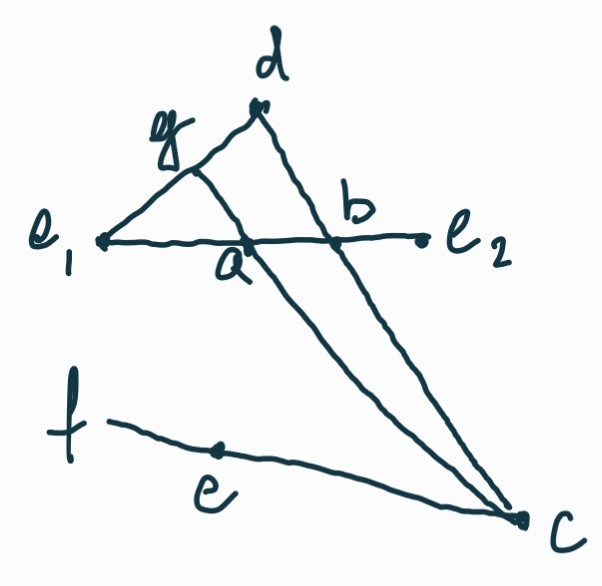
\includegraphics[width=0.5\textwidth]{tempimages/DistinctAndMixture.jpg}
\end{figure}

\begin{proof}
	Let $\ens \distinct \ens[a] = p \ens_1 + \bar{p} \ens_2$ for some $p \in (0, 1)$. Let $\ens[b] = \alpha \ens_1 + \bar{\alpha} \ens_2$ with $0 \leq \alpha < p$. We can do so without loss of generality since switching $\ens_1$ with $\ens_2$ would lead to the case where $1 \geq \alpha > p$. Suppose $\ens[b]$ is not distinct from $\ens$. Then we can find $\ens[c] \in \Ens$ such that $\ens[b] = \beta \ens[c] + \bar{\beta} \ens[d]$ and $\ens = \gamma \ens[c] + \bar{\gamma} \ens[f]$ for some $\ens[d], \ens[f] \in \Ens$ and $\beta, \gamma \in (0, 1)$.
	
	Setting $\epsilon = \frac{p - \alpha}{\bar{\alpha}}$ and $\lambda = \bar{\epsilon} \beta$ we have:
	\begin{align*}
		\ens[a] &= p \ens_1 + \bar{p} \ens_2 = \left(p - \frac{\bar{p}}{\bar{\alpha}} \alpha \right) \ens_1 + \frac{\bar{p}}{\bar{\alpha}} \alpha \ens_1 + \frac{\bar{p}}{\bar{\alpha}} \bar{\alpha}\ens_2 \\
		&= \left(\frac{p\bar{\alpha} - \bar{p}\alpha}{\bar{\alpha}} \right) \ens_1 + \frac{\bar{p}}{\bar{\alpha}} (\alpha \ens_1 + \bar{\alpha} \ens_2) = \left(\frac{p - p\alpha - \alpha + p \alpha}{\bar{\alpha}} \right) \ens_1 + \frac{1 - p + \alpha - \alpha}{\bar{\alpha}} (\alpha \ens_1 + \bar{\alpha} \ens_2) \\
		&= \frac{p - \alpha}{\bar{\alpha}}  \ens_1 + \left( 1 - \frac{p - \alpha}{\bar{\alpha}}\right) (\alpha \ens_1 + \bar{\alpha} \ens_2) = \epsilon \ens_1 + \bar{\epsilon} (\alpha \ens_1 + \bar{\alpha} \ens_2) = \epsilon \ens_1 + \bar{\epsilon} \ens[b] \\
		&= \epsilon \ens_1 + \bar{\epsilon} ( \beta \ens[c] + \bar{\beta} \ens[d] ) = \bar{\epsilon} \beta \ens[c] + \epsilon \ens_1 + \bar{\epsilon} \bar{\beta} \ens[d] = \lambda \ens[c] + \bar{\lambda} \ens[g]
	\end{align*}
	where $\ens[g] = \frac{1}{\bar{\lambda}}\left( \epsilon \ens_1 + \bar{\epsilon} \bar{\beta} \ens[d] \right)$. This means $\ens[a]$ and $\ens$ have a common component, which is a contradiction. Therefore $\ens[b] \distinct \ens$ and $\ens \distinct p \ens_1 + \bar{p} \ens_2$ for all $p \in [0, 1]$
	
	As a counter-example for the converse, consider a circle and three points on the circumference. These are all distinct from each other. Now take two points. A mixture will be on the chord that connects the two. Connecting any mixture with the third point will give a line that will intersect the circumference at a fourth point. This means that the given mixture is has a common component with the third point, even though the third point is distinct from the first two.	
\end{proof}

\begin{remark}
	Note that, in classical mechanics, $\ens \distinct p \ens_1 + \bar{p} \ens_2$ for some $p$ does imply that $\ens \distinct \ens_1$ and $\ens \distinct \ens_2$. However, this is not the case in quantum mechanics. For example, consider the Bloch sphere and the states $x^+$, $x^-$, $z^+$, and $z^-$. These are all distinct ensembles. We have $\frac{1}{2} x^+ + \frac{1}{2} x^- = \frac{1}{2} z^+ + \frac{1}{2} z^-$. Therefore a mixture of $x^+$ and $x^-$ has a common component with $z^+$.
\end{remark}

\begin{defn}
	 Let $\ens[\rho] = p \ens_1 + \bar{p} \ens_2$ with $p \in (0,1)$. Then we say that $\ens_2$ is a $p$-\textbf{complement} of $\ens_1$ towards $\ens[\rho]$. An ensemble space is \textbf{complemented} if all $p$-complements are unique for all $p \in (0, 1)$.
\end{defn}

\begin{prop}\label{pm_es_complementedIsVectorSpace}
	An ensemble space is complemented if and only if it is a convex subset of a real vector space for which mixtures are linear combination.
\end{prop}
\begin{proof}
	Theorem 4 in \url{https://arxiv.org/abs/1105.1270} states that a convex space embeds into a real vector space with $c_\lambda(x,y) = \lambda x + \bar{\lambda}y$ if and only if
	$$ c_\lambda(x,y) = c_\lambda(x,z) \; \forall \lambda \in (0,1) \implies y = z.$$ This is exactly the condition that the $\lambda$-complement is unique.
\end{proof}

\begin{prop}
	Discrete classical ensemble spaces, continuous classical ensemble spaces and quantum ensemble spaces satisfy the axiom of mixture and are complemented ensemble spaces.
\end{prop}

\begin{proof}
	The space of probability measures, discrete or continuous, $\Ens$ is a convex subset of the vector space of finite signed measures. This means that it is closed under convex combinations: $\sum p_i \ens_i$ for all $\{e_i\} \subseteq \Ens$ and $\sum p_i = 1$. The properties of mixing are inherited from the properties of linear combinations. Therefore the discrete and continuous classical ensemble spaces satisfy the axiom of mixture. Moreover, $\Ens$ is a convex subset of a vector space, it is complemented by proposition \ref{pm_es_complementedIsVectorSpace}.
	
	Similarly, the space of positive semi-definite self-adjoint operators with trace one is a convex subset of the vector space of self-adjoint operators. Therefore it is closed under convex combinations and it will satisfy the axiom of mixture. Moreover, it is complemented convex by proposition \ref{pm_es_complementedIsVectorSpace}.
\end{proof}


\begin{remark}
	Since all current physical ensemble spaces are complemented, it is not yet clear whether an ensemble space must be complemented or not. It is difficult to justify as it is a claim on existence of more refined ensembles. It may very well be that this is just an assumption on the decomposition, which may fail in new physical conditions (e.g. at Planck scale). It may also be something that the strict concavity of the entropy requires.
\end{remark}


\section{Entropy}

\begin{defn}
	Given the coefficients $\{p_i\} \in [0,1]$ such that $\sum p_i = 1$, the \textbf{entropy of the coefficients} (also known as Shannon entropy) is defined as $I(\{p_i\}) = - \sum p_i \log p_i $.
\end{defn}

\begin{axiom}[Axiom of entropy]
	An ensemble space $\Ens$ is equipped a a function $S : \Ens \to \mathbb{R}$ called \textbf{entropy} with the following properties
	\begin{itemize}
		\item \textbf{Continuity}
		\item \textbf{Strict concavity}: $S(p_1\ens_1 + p_2 \ens_2) \geq p_1 S(\ens_1) + p_2 S(\ens_2)$ with the equality holding if and only if $\ens_1 = \ens_2$
		\item \textbf{Upper variability bound}: $S(p_1\ens_1 + p_2 \ens_2) \leq I(p_1, p_2) + p_1 S(\ens_1) + p_2 S(\ens_2)$; if the equality hold then, $e_1$ and $e_2$ are \textbf{disjunct}, noted $e_1 \disjunct e_2$
	\end{itemize}
\end{axiom}

\begin{justification}
	The entropy quantifies the variability of the elements within the ensemble. This justifies the existence of the entropy.
	
	Small changes in the ensemble should produce small changes in the variability, which justifies continuity. Mixing different ensembles will increase the variability, which justifies concavity. Mixing the same ensemble, however, should not increase the variability, which justifies strict concavity. 
	
	The variability increase is maximal when the two ensembles are disjunct, meaning they have no elements in common. In this case, the increase in variability is given only by the coefficients and must follow the Shannon entropy as it is the only continuous indicator of variability that is linear in probability. This justifies the upper bound.
\end{justification}

\begin{remark}
	In \url{https://arxiv.org/abs/1912.02012} we showed how the Shannon entropy quantifies the variability of elements within a distribution. Is it possible to rederive $I$ from requirements on convex spaces instead of distributions in particular? This would make the axiom less ad-hoc.
\end{remark}


\begin{axiom}[Axiom of entropic disjunctness]
	The entropy function of an ensemble space obeys the following properties
	\begin{itemize}
		\item \textbf{Disjunctness implies distinctness}: $\ens_1 \disjunct \ens_2$ implies $\ens_1 \distinct \ens_2$
		\item \textbf{Mixtures preserve disjunctness}: let $\ens_1 = p \ens_2 + \bar{p} \ens_3$, then $\ens_4 \disjunct \ens_1$ if and only if $\ens_4 \disjunct \ens_2$ and $\ens_4 \disjunct \ens_3$
	\end{itemize}
\end{axiom}

\begin{justification}
	If two ensembles are disjunct, they have no elements in common. Therefore there will be no common component with the two. We are justified to assume that disjunctness implies distinctness.
	
	Suppose an ensemble $\ens_1$ is disjunct from the mixture of two ensembles $\ens_2$ and $\ens_3$. That it has no elements in common with the mixture, which means it has no elements in common with either of them. Therefore $\ens_1$ is disjunct from both $\ens_2$ and $\ens_3$. Now suppose $\ens_1$ is disjunct from both $\ens_2$ and $\ens_3$. That it means it has no elements in common with either of them, and therefore it does not have any elements in common with their mixture. Therefore $\ens_1$ is disjunct from the mixture of two ensembles $\ens_2$ and $\ens_3$. We are justified to assume that mixtures preserve disjunctness.
\end{justification}

\begin{remark}
	It is unclear whether or not these properties can be proven by the axiom of mixture. It is possible to prove that two disjunct ensembles are not one the component of the other. The entropy of the coefficients (i.e. the Shannon entropy) has a vertical asymptote at each end. If two elements are disjunct, the entropy along the segment that connects the two follows that function plus a linear function, which does not change the vertical asymptotes. Therefore the segment cannot be extended while preserving the convexity of the entropy, and therefore the two distinct elements must the extremes of the line that connects the two. This is necessary for distinctness, but not sufficient. Maybe, extending the argument, one can at least prove that disjunctness implies distinctness.
\end{remark}

\begin{prop}
	The discrete classical ensemble spaces, continuous classical ensemble spaces and quantum ensemble spaces satisfies the axiom of mixture and the axiom of entropic disjunctness.
\end{prop}

\begin{proof}
	In both classical cases, the entropy is a function of only the probabilities of the decomposition in terms of pure states. The function is continuous in terms of those variables as $x \log x$ is a continuous function. [TODO find short proof of convexity and maximum bound]
	
	In the quantum case, the entropy is a continuous function of the density operator as the trace, multiplication and logarithm of an operator are all continuous functions. [TODO find short proof of convexity and maximum bound]
\end{proof}

\begin{remark}
	There should be an interplay between convexity and entropy which limits either the space or the possible entropy. For example, consider a line. It is a convex space with no extreme points. We can parameterize the space with a variable $x$ such that the mixture of two ensembles is identified by the average $x$. Entropy can be written as $S(x)$. Since $S(x)$ is strictly concave over an infinite range, it will tend to minus infinity either when $x$ tends to infinity or minus infinity. Now take a line that intersects the curve. This will intersect it at only two points. By strict convexity, there is only going to be a single point with maximum vertical distance to the line, which has to be greater than zero. Now imagine moving the line down by one vertical unit. The vertical distance now is greater than one. This means that the average entropy can increase more than one during mixture, which violates the upper variability bound. Therefore a line cannot be an ensemble space.
	
	Note that an open segment is absolutely fine. We can, in fact, imagine a two state discrete classical ensemble space with the endpoint removed. This suggests that the convex space knows something about the geometry (probably parallelism and ratio of length - i.e. the affine structure).
\end{remark}

\begin{conj}
	Let $\ens_1, \ens_2 \in \Ens$ be such that $p\ens + \bar{p} \ens_1 = p\ens + \bar{p} \ens_2$ for some $p \in (0, 1)$ and $\ens \in \Ens$. Then $\ens_1$ and $\ens_2$ are not disjunct.
\end{conj}

\begin{remark}
	It seems very unlikely that differences in states that can be obscured by mixing would correspond to disjunct states. The more general question is whether the strict concavity of the entropy allows non-complemented spaces.
\end{remark}

\begin{defn}
	Two sets of ensembles $U, V \subseteq \Ens$ are disjunct if $\ens_1 \disjunct \ens_2$ for all $\ens_1 \in U$ and $\ens_2 \in V$. 
\end{defn}


\begin{defn}
	An ensemble space $\Ens$ is \textbf{reducible} (or \textbf{classical}) if distinct ensembles are also disjunct. That is, $\ens_1 \distinct \ens_2$ implies $\ens_1 \disjunct \ens_2$.
\end{defn}

\begin{justification}
	Given that $\ens_1 \disjunct \ens_2$ implies $\ens_1 \distinct \ens_2$, classical spaces add the opposite implication. Therefore they exclude the case where two ensembles are disjunct but not distinct. This case describes two ensembles that have elements in common, but there is no ensemble corresponding to those common elements. That is, we cannot refine the ensembles into three distinct ones: one with only elements of the first, one with only elements of the second and one with elements of both. In other words, we cannot reduce the coarser description of the system into finer distinct descriptions. In the excluded case, then, the coarser description is irreducible into finer ensembles. This justifies the definition.
	
	As we prove below, that case does not exist in classical mechanics, but exists in quantum mechanics. This justifies calling the property classical.
\end{justification}

\begin{remark}
	The above property should ultimately be responsible for the single decomposition in terms of pure states.
\end{remark}

\begin{prop}
	Continuous and discrete classical ensemble spaces are reducible.
\end{prop}

\begin{proof}
	In both cases, ensembles are probability measures: the first over the Borel algebra of a symplectic manifold; the second over the power set of countably many elements. In both cases, the upper bound of the entropy is maximized if and only if the probability measures being combined have disjoint support. This means that two ensembles are disjunct if and only if the respective probability measures have disjoint support. Intuitively, two probability distributions can have a common sub-distribution if and only if they overlap. Therefore two ensembles representing probability measures with disjoint support are exactly ensembles that are distinct. Therefore, in both cases, the ensemble space is reducible.
\end{proof}

\section{Dimension of a set of ensembles}

\begin{prop}[Exponential entropy subadditivity]\label{pm_es_exponentialEntropySubadditivity}
	Let $\ens_1, \ens_2 \in \Ens$. Let $S_1 = S(\ens_1)$ and $S_2 = S(\ens_2)$. Let $\ens = p \ens_1 + \bar{p} \ens_2$ for some $p \in [0,1]$ and $S = S(\ens)$. Then $2^S \leq 2^{S_1} + 2^{S_2}$, with the equality if and only if $\ens_1$ and $\ens_2$ are disjunct and $p = \frac{2^{S_1}}{2^{S_1} + 2^{S_2}}$.
\end{prop}

\begin{proof}
	If $p$ is fixed, the upper variability bound of entropy is saturated only if $\ens_1$ and $\ens_2$ are disjunct by definition. The entropy maximum for the mixed ensemble can only be achieved when the elements are disjunct, for some value of $p$.
	
	Now fix $S_1$ and $S_2$. The entropy of the mixture depends only on $p$, so we need to find the $p$ that maximizes the expression.
	\begin{equation}
		\begin{aligned}
			0 = \frac{dS}{dp} &= \frac{d}{dp} S(\ens) =\frac{d}{dp} \left( - p \log p - \bar{p} \log \bar{p} + p S_1 + \bar{p} S_2 \right) \\
			&= - \log p - 1 + \log \bar{p} + 1 + S_1 - S_2 \\
			\log \frac{p}{\bar{p}} &= \log 2^{S_1} - \log 2^{S_2} \\
			\log \frac{p}{1-p} &= \log \frac{2^{S_1}}{2^{S_2}}  \\
			p 2^{S_2} &= (1-p) 2^{S_1}  \\
			p (2^{S_1} + 2^{S_2}) &= 2^{S_1}  \\
			p &= \frac{2^{S_1}}{2^{S_1} + 2^{S_2}}  \\
		\end{aligned}
	\end{equation}
	Having found the value of $p$ that maximizes the entropy, we can calculate the maximum entropy.
	\begin{equation}
	\begin{aligned}
		\bar{p} &= 1- \frac{2^{S_1}}{2^{S_1} + 2^{S_2}} = \frac{2^{S_2}}{2^{S_1} + 2^{S_2}} \\
		S &= S(\ens) = - p \log p - \bar{p} \log \bar{p} + p S_1 + \bar{p} S_2  \\
		&= - \frac{2^{S_1}}{2^{S_1} + 2^{S_2}} \log \frac{2^{S_1}}{2^{S_1} + 2^{S_2}} - \frac{2^{S_2}}{2^{S_1} + 2^{S_2}} \log \frac{2^{S_2}}{2^{S_1} + 2^{S_2}} \\
		&+ \frac{2^{S_1}}{2^{S_1} + 2^{S_2}} \log 2^{S_1} + \frac{2^{S_2}}{2^{S_1} + 2^{S_2}} \log 2^{S_2} \\
		&= \frac{2^{S_1}}{2^{S_1} + 2^{S_2}} \log \left( 2^{S_1} + 2^{S_2} \right) + \frac{2^{S_2}}{2^{S_1} + 2^{S_2}} \log \left( 2^{S_1} + 2^{S_2} \right) \\
		&= \frac{2^{S_1} + 2^{S_2}}{2^{S_1} + 2^{S_2}} \log \left( 2^{S_1} + 2^{S_2} \right) \\
		\log 2^S &= \log \left( 2^{S_1} + 2^{S_2} \right) \\
		2^S &=  2^{S_1} + 2^{S_2}  \\
	\end{aligned}
	\end{equation}
	Therefore the maximum entropy obtainable through a mixture is $S = \log (2^{S_1} + 2^{S_2})$ which is obtained when $\ens_1$ and $\ens_2$ are disjunct and $p = \frac{2^{S_1}}{2^{S_1} + 2^{S_2}}$.
\end{proof}

\begin{defn}
	Let $U \subseteq \Ens$ be the subset of an ensemble space. The \textbf{convex hull} of $U$, noted $\hull(U)$ is the set of all possible mixtures that can be constructed with elements contained in $U$.
\end{defn}

\begin{coro}
	The convex hull has the following properties
	\begin{enumerate}
		\item $U \subseteq \hull(U)$
		\item $U \subseteq V \implies \hull(U) \subseteq \hull(V)$
		\item $\hull(\hull(U)) = \hull(U)$
	\end{enumerate}
	and is therefore a closure operation
\end{coro}

\begin{proof}
	1. Every element of $U$ is trivially a mixture of elements of $U$. Therefore $U \subseteq \hull(U)$.
	
	2. Let $\ens \in \hull(U)$. Then it is a mixture of some elements of $U$. Since $U \subseteq V$, then $\ens$ is also the mixture of some elements of $V$ and therefore $\ens \in \hull(V)$.
	
	3. Since mixing is associative and commutative, a mixture of mixtures of $U$ can be reepressed as a mixture of $U$. Therefore for all $\ens \in \hull(\hull(U))$ we have $\ens \in \hull(U)$.
\end{proof}

\begin{defn}
	Let $U \subseteq \Ens$ be the subset of an ensemble space. The \textbf{dimension} of $U$ is defined as $\dim(U) = \sup(2^{S(\hull(U))})$ if $U \neq \emptyset$ and $\dim(U) = 0$ otherwise.
\end{defn}

\begin{prop}
	The dimension is a set function that is
	\begin{enumerate}
		\item non negative: $\dim(U) \in [0, +\infty]$
		\item monotone: $U \subseteq V \implies \dim(U) \leq \dim(V)$
		\item subadditive: $\dim(U \cup V) \leq \dim(U) + \dim(V)$
		\item additive over disjunct sets: $U \disjunct V \implies \dim(U \cup V) = \dim(U) + \dim(V)$ 
	\end{enumerate}
\end{prop}

\begin{proof}
	1. The dimension takes a subset of $\Ens$ and returns a real value and is therefore a set function. The exponential can only return non-negative values, therefore the dimension of a set is non-negative. 
	
	2. Let $U, V \subseteq \Ens$ such that $U \subseteq V$. If $U = \emptyset$, we have $\dim(U) = 0$. Since $\dim(V)$ is non-negative, $\dim(U) \leq \dim(V)$. If $U \neq \emptyset$, $\hull(U) \subseteq \hull(V)$ and therefore $2^{S(\hull(U))} \subseteq 2^{S(\hull(V))}$. This means that the supremum of the first set cannot be greater than the supremum of the second set, and therefore $\dim(U) \leq \dim(V)$. The dimension is a monotone set function.
	
	3. Let $U, V \subseteq \Ens$ and let $\ens \in \hull(U \cup V)$. Then we can write $\ens = p \ens[u] + \bar{p} \ens[v]$ for some $p \in [0,1]$, $\ens[u] \in U$ and $\ens[v] \in V$. By \ref{pm_es_exponentialEntropySubadditivity} and the definition of dimension, $2^{S(\ens)} = 2^{S(\ens[u])} + 2^{S(\ens[v])} \leq \dim(U) + \dim(V)$. Since this is true for any element of $\hull(U \cup V)$, the supremum of the exponential entropy cannot exceed the sum of the dimensions. Therefore $\dim(U \cup V) \leq \dim(U) + \dim(V)$, the dimension is subadditive.
	
	4. Let $U, V \subseteq \Ens$ be two disjunct subsets. Let $\{\ens[u]_i\} \subset U$ be a sequence of ensembles such that $2^{S(\ens[u]_i)} \to \dim(U)$ and let $\{\ens[v]_i\} \subset V$ be a sequence of ensembles such that $2^{S(\ens[v]_i)} \to \dim(V)$. Consider $\ens_i = p_i \ens[u]_i + \bar{p_i} \ens[v]_i$ where $p_i = \frac{2^{S(\ens[u]_i)}}{2^{S(\ens[u]_i)} + 2^{S(\ens[v]_i)}}$. Then, by \ref{pm_es_exponentialEntropySubadditivity}, $2^{S(\ens_i)} = 2^{S(\ens[u]_i)} + 2^{S(\ens[v]_i)}$. This means that $2^{S(\ens_i)} \to \dim(U) + \dim(V)$. Therefore $\dim(U \cup V) \geq \dim(U) + \dim(V)$. Combining with the previous result, $\dim(U \cup V) = \dim(U) + \dim(V)$. Therefore dimension, as set function, is additive over disjunct sets of ensembles.
\end{proof}

\section{Entropic geometry}

We now show that entropy imposes a geometric structure on the ensemble space.

\begin{defn}
	Given two ensembles $\ens_1, \ens_2 \in \Ens$, the \textbf{mixing entropy}, also called Jensen-Shannon divergence, is the increase in entropy associated to their mixture. That is:
	$$MS(\ens_1, \ens_2) = S\left(\frac{1}{2}\ens_1 + \frac{1}{2} \ens_2\right) - \left(\frac{1}{2} S(\ens_1) + \frac{1}{2} S(\ens_2)\right).$$
\end{defn}

\begin{coro}
	The mixing entropy obeys the following bounds
	$$ 0 \leq MS(\ens_1, \ens_2) \leq 1.$$
	The lower bound is satisfied if and only if $\ens_1 = \ens_2$ and the upper bound is satisfied if and only if $\ens_1 \disjunct \ens_2$.
\end{coro}

\begin{proof}
	The bounds descend directly from the bounds on entropy. By strict concavity, $S(p_1\ens_1 + p_2 \ens_2) \geq p_1 S(\ens_1) + p_2 S(\ens_2)$, which means $S(p_1\ens_1 + p_2 \ens_2) - p_1 S(\ens_1) - p_2 S(\ens_2) \geq 0$, and in particular $S(\frac{1}{2} \ens_1 + \frac{1}{2} \ens_2) - \frac{1}{2} S(\ens_1) - \frac{1}{2} S(\ens_2) = MS(\ens_1, \ens_2) \geq 0$. By strict concavity, the equality holds if and only if $\ens_1 = \ens_2$
	
	By the upper variability bound, $S(p_1\ens_1 + p_2 \ens_2) \leq I(p_1, p_2) + p_1 S(\ens_1) + p_2 S(\ens_2)$, which means $S(p_1\ens_1 + p_2 \ens_2) - p_1 S(\ens_1) - p_2 S(\ens_2) \leq I(p_1, p_2)$, and in particular $S(\frac{1}{2} \ens_1 + \frac{1}{2} \ens_2) - \frac{1}{2} S(\ens_1) - \frac{1}{2} S(\ens_2) = MS(\ens_1, \ens_2) \leq I(\frac{1}{2}, \frac{1}{2}) = 1$. Given that $\ens_1$ and $\ens_2$ are disjunct by definition if they saturate the upper variability bound, the equality holds if and only if $\ens_1$ and $\ens_2$ are disjunct.
\end{proof}

\begin{prop}
	In discrete and continuous classical cases, the mixing entropy coincides with the Jensen-Shannon divergence. In quantum spaces it coincindes with the quantum Jensen-Shannon divergence.
\end{prop}

\begin{proof}
	Looking at the definitions, for example at \url{https://en.wikipedia.org/wiki/Jensen%E2%80%93Shannon_divergence}, one can see that
	$$ JSD(\ens_1, \ens_2) = S\left(\frac{1}{2}\ens_1 + \frac{1}{2}\ens_2 \right)  - \frac{1}{2} \left(S(\ens_1) + S(e_2)\right) = MS(\ens_1, \ens_2)$$.
	The same is true for the quantum case:
	$$ QJSD(\ens_1, \ens_2) = S\left(\frac{1}{2}\ens_1 + \frac{1}{2}\ens_2 \right)  - \frac{1}{2} \left(S(\ens_1) + S(\ens_2)\right) = MS(\ens_1, \ens_2)$$.
\end{proof}

\begin{defn}
	An ensemble space is \textbf{geometric} if it is complemented and has a twice differentiable entropy with respect to the mixing coefficients.
\end{defn}

\begin{coro}
	A geometric ensemble space is a convex subset of a smooth vector space.
\end{coro}

\begin{proof}
	Since a geometric ensemble space is complemented, it embeds into a real vector space. The differentiable structure is imposed by requiring that any parameter used to define families of ensembles must be twice differentiable with respect to the entropy.
\end{proof}

\begin{remark}
	The above restriction is useful to use notion of standard differential geometry. It may be that some of the results can be generalized: differentiability of the entropy may be derived by continuity, concavity of the entropy and differentiability of $I(p_1, p_2)$; it may be that the convex structure may be enough to define a generalized version of tangent space. This would should be the target of future research.
\end{remark}

\begin{defn}
	Let $V \subseteq \Ens$ be a finite dimensional subregion of a geometric ensemble space. Let $\ens \in \Ens$ be an ensemble, the \textbf{tangent space} at $\ens$, noted $T_{\ens}$, is the space of all infinitesimal variations $\delta \ens$. The \textbf{norm} of a variation $\delta \ens \in T_{\ens}$ is given by
	$$ \lVert \delta \ens \rVert_{\ens} = \sqrt{ MS(\ens, \ens + \delta \ens) }.$$
	The \textbf{metric tensor} (i.e. the inner product between two variations $\delta \ens_1 , \delta \ens_2 \in T_{\ens}$ ) is given by
	$$ g_{\ens}( \delta \ens_1, \delta \ens_2 ) = \frac{1}{2} \left( \lVert \delta \ens_1 + \delta \ens_2 \rVert_{\ens}^2 - \lVert \delta \ens_1 \rVert_{\ens}^2 - \lVert \delta \ens_2 \rVert_{\ens}^2 \right).$$
\end{defn}

\begin{thrm}
	Let $\Ens$ be a geometric ensemble space and $V \subseteq \Ens$ a finite dimensional subregion. Then
	$$ \lVert \delta \ens \rVert_{\ens}^2 = - \frac{1}{8} \frac{\partial^2 S}{\partial \ens^2}(\delta \ens , \delta \ens) $$
	and 
	$$ g_{\ens}( \delta \ens_1, \delta \ens_2 ) = - \frac{1}{8} \frac{\partial^2 S}{\partial \ens ^2}( \delta \ens_1, \delta \ens_2 ).$$
	Then $V$ is a Riemannian manifold with $g_{\ens}$ as the metric tensor and $\lVert \cdot \rVert_{\ens}$ as the norm.
\end{thrm}

\begin{proof}
	To recover the first two expression, we simply have to calculate the leading term. Since the entropy is twice differentiable, we can expand it as
\begin{equation}
	\begin{aligned}
		S(\ens + \delta \ens) &= S(\ens) + \frac{\partial S}{\partial \ens} \delta \ens + \frac{1}{2} \frac{\partial^2 S}{\partial \ens^2} \delta \ens \delta \ens + O(\delta \ens ^3).
	\end{aligned}
\end{equation}
Expanding the definition of $MS$, we have
\begin{equation}
	\begin{aligned}
		MS(\ens, \ens + \delta \ens) &= S\left(\frac{1}{2} \ens + \frac{1}{2}(\ens + \delta \ens) \right) - \frac{1}{2} S(\ens) - \frac{1}{2} S(\ens+\delta \ens) \\
		&=  S\left(\ens + \frac{1}{2} \delta \ens \right) - \frac{1}{2} S(\ens) - \frac{1}{2} S(\ens+\delta \ens) \\
		&= S(\ens) + \frac{\partial S}{\partial \ens} \frac{1}{2}\delta \ens + \frac{1}{2} \frac{\partial^2 S}{\partial \ens^2} \frac{1}{2}\delta \ens \frac{1}{2}\delta \ens + O(\delta \ens ^3) \\
		&- \frac{1}{2} S(\ens) - \frac{1}{2} \left( S(\ens) + \frac{\partial S}{\partial \ens} \delta \ens + \frac{1}{2} \frac{\partial^2 S}{\partial \ens^2} \delta \ens \delta \ens + O(\delta \ens ^3) \right) \\
		&= S(\ens) + \frac{1}{2} \frac{\partial S}{\partial \ens} \delta \ens + \frac{1}{8} \frac{\partial^2 S}{\partial \ens^2} \delta \ens \delta \ens \\
		&- S(\ens) - \frac{1}{2} \frac{\partial S}{\partial \ens} \delta \ens - \frac{1}{4} \frac{\partial^2 S}{\partial \ens^2} + O(\delta \ens ^3) \\
		&= - \frac{1}{8} \frac{\partial^2 S}{\partial \ens^2} \delta \ens \delta \ens + O(\delta \ens ^3).
	\end{aligned}
\end{equation}

Therefore
$$ \lVert \delta \ens \rVert^2 = MS(\ens, \ens + \delta \ens) = - \frac{1}{8} \frac{\partial^2 S}{\partial \ens^2} (\delta \ens, \delta \ens).$$

We can now substitute the norm to the definition of metric tensor. We have
\begin{equation}
	\begin{aligned}
		g_{\ens}(\delta \ens_1, \delta \ens_2 ) &= \frac{1}{2} \left( \lVert \delta \ens_1 + \delta \ens_2 \rVert^2 - \lVert \delta \ens_1 \rVert^2 - \lVert \delta \ens_2 \rVert^2 \right) \\
		&= \frac{1}{2} \left( - \frac{1}{8} \frac{\partial^2 S}{\partial \ens^2} (\delta \ens_1 + \delta \ens_2, \delta \ens_1 + \delta \ens_2) + \frac{1}{8} \frac{\partial^2 S}{\partial \ens^2} (\delta \ens_1, \delta \ens_1) +\frac{1}{8} \frac{\partial^2 S}{\partial \ens^2} (\delta \ens_2, \delta \ens_2) \right) \\
		&= - \frac{1}{16} \left(  \frac{\partial^2 S}{\partial \ens^2} (\delta \ens_1, \delta \ens_1) + \frac{\partial^2 S}{\partial \ens^2} (\delta \ens_1, \delta \ens_2) + \frac{\partial^2 S}{\partial \ens^2} (\delta \ens_2, \delta \ens_1) + \frac{\partial^2 S}{\partial \ens^2} (\delta \ens_2, \delta \ens_2) \right. \\
		&-  \left. \frac{\partial^2 S}{\partial \ens^2} (\delta \ens_1, \delta \ens_1) - \frac{\partial^2 S}{\partial \ens^2} (\delta \ens_2, \delta \ens_2) \right) \\
		&= - \frac{1}{8} \frac{\partial^2 S}{\partial \ens^2} (\delta \ens_1, \delta \ens_2) \\
	\end{aligned}
\end{equation}

	Let us now take a finite dimensional region $V \subseteq \Ens$. Since $V$ is a finite dimensional subregion of a real vector space, it will be a manifold. It will have a smooth structure inherited from the ensemble space.
	
	Let us now show that $g$ is a metric tensor. Restricted to $V$, $g|_V$ is the Hessian of the entropy $S$. Therefore it is a symmetric rank two tensor which means a symmetric bilinear function of the arguments. Since the entropy is strictly concave, the Hessian is negative definite and therefore $g$ is positive definite. Therefore $(V, g|_V)$ is a Riemannian manifold.
\end{proof}

\begin{conj}
	The mixing entropy is the square of a distance function.
\end{conj}

\begin{proof}
	This should follow as it is the distance induced by the metric.
\end{proof}

\begin{remark}
	We have shown that, under very general conditions, a generalized ensemble space is a geometric space, where the notion of distance and angle are fully defined by the entropy. That is, all geometric structures in physics are entropic structures.

	The metric we find is the \href{https://en.wikipedia.org/wiki/Fisher_information_metric}{Fisher-Rao metric}, whose action/curve length is liked to the \href{https://en.wikipedia.org/wiki/Fisher_information_metric#Relation_to_the_Jensen%E2%80%93Shannon_divergence}{Jensen-Shannon divergence}. The factor of 8 may have to be fixed. What we have is a generalization of those results, which applies to both classical and quantum mechanics as a special case.

	We are also working on a notion of derivative/differentiability that requires just a topological space that is locally isomorphic to a vector space, regardless of dimensionality. This can be used as a basic framework to work directly on the full ensemble space, instead on finite dimensional subsets.
\end{remark}

\section{Ensemble subspaces}

We now want to define a notion of subspace in a way that recovers the notions of subspaces we have in both classical and quantum mechanics. Given that orthogonality in all three cases corresponds to ensembles being disjunct, disjunct ensembles will need to belong to different subspaces. The idea is to reconstruct subspaces only from the disjunct relationship.

\subsection{Irreflexive symmetric relations and topped $\cap$-structures}

We will first prove a more general set of results, on a generic set (not necessarily an ensemble space) with an irreflexive symmetric relation (not necessarily disjunctness of ensembles). This will give us a more general tool to investigate possible different notion of subspaces.

\begin{defn}
	Let $X$ be a set and $R \subseteq X \times X$ a symmetric relation. Given a subset $U \subseteq X$, we define the \textbf{$R$-complement} to be
	$$ U^{RC} = \{ a \in X \, | \, \forall b \in U, aRb  \}. $$
\end{defn}

\begin{prop}\label{pm_es_rComplProps}
	Let $X$ be a set and $R \subseteq X \times X$ a symmetric relation. Then:
	\begin{enumerate}
		\item $U \subseteq V \implies V^{RC} \subseteq U^{RC}$
		\item $U \subseteq (U^{RC})^{RC}$
		\item $U^{RC} = ((U^{RC})^{RC})^{RC}$
		\item $U^{RC} = (V^{RC})^{RC} \iff (U^{RC})^{RC} = V^{RC}$
		\item $(\bigcup_{i \in I} U_i )^{RC} = \bigcap_{i \in I} (U_i)^{RC}$
		\item $\emptyset^{RC} = X$
	\end{enumerate}
\end{prop}

\begin{proof}
	1. Suppose $a \in V^{RC}$. Then, by definition, $\forall b \in V, aRb$. Since $U \subset V$, it is also true that $\forall b \in U, aRb$. Therefore $a \in U^{RC}$ by definition. Since $a$ was arbitrary, $V^{RC} \subseteq U^{RC}$.
	
	2. By expanding the definition of complement, we have $(U^{RC})^{RC}=\{ a \in X \, | \, \forall b \in U^{RC}, aRb \} = \{ a \in X \, | \, \forall b \in \{ c \in X \, | \, \forall d \in U, cRd  \}, aRb \} = \{ a \in X \, | \, \forall b \in X \, s.t. (\forall d \in U, bRd), aRb \}$.
	
	Let $a \in U$ and let $b \in X$ such that $\forall d \in U, bRd$. Since $a \in U$ and $bRd$ for all $b \in U$, we have $bRa$ in particular. Since $R$ is symmetric, $aRb$. Given that $b$ was arbitrary, we conclude that $\forall b \in X \, s.t. (\forall d \in U, bRd), aRb$. Therefore $a \in (U^{RC})^{RC}$ by definition of complement. Given that $a$ was arbitrary, $U \in (U^{RC})^{RC}$.
	
	3. We again expand the definition and have $((U^{RC})^{RC})^{RC} = \{ a \in X \, | \, \forall b \in (U^{RC})^{RC}, aRb \}$.
	
	Let $x \in ((U^{RC})^{RC})^{RC}$. Then $\forall b \in (U^{RC})^{RC}, xRb$ by definition of the complement. Since by 1. $U \subset (U^{RC})^{RC}$, we can restrict the previous expression to only the elements of $U$, and therefore $\forall b \in U, xRb$. But this means that $x \in U^{RC}$ by definition of the complement. Since $x$ was arbitrary, $((U^{RC})^{RC})^{RC} \subseteq U^{RC}$. But by 1., we also have $U^{RC} \subseteq ((U^{RC})^{RC})^{RC}$ since $U^{RC}$ is just a set onto which we can apply the complement twice . By two-way containment, we have $U^{RC} = ((U^{RC})^{RC})^{RC}$.
	
	4. Let $U, V \subseteq X$ such that $U^{RC} = (V^{RC})^{RC}$. Applying the complement on each side, $(U^{RC})^{RC} = ((V^{RC})^{RC})^{RC}$. By the previous property $((V^{RC})^{RC})^{RC} = V^{RC}$ and therefore $(U^{RC})^{RC} = V^{RC}$. Switching $U$ and $V$ proves the other direction.
	
	5. We have:
	\begin{equation*}
		\begin{aligned}
		(\bigcup_{i \in I} U_i )^{RC} &= \{ a \in X \, | \, \forall b \in \bigcup_{i \in I} U_i, aRb \} \\
		&= \{ a \in X \, | \, \forall U_i, \forall  b \in U_i, aRb \} \\
		&= \{ a \in X \, | \, \forall U_i, a \in \{ c \in X \, | \,  \forall  b \in U_i, cRb \} \} \\
		&= \bigcap_{i \in I} \{ c \in X \, | \, \forall  b \in U_i, cRb\} \\
		&= \bigcap_{i \in I} (U_i)^{RC}
	\end{aligned}
	\end{equation*}
	Note that this property does not rely on the symmetry of $R$.
	
	6. Let $a \in X$. There is no $b \in \emptyset$ such that $aRb$. Therefore $\forall b \in \emptyset, aRb$. This means that $a \in \emptyset^{RC}$. Since $a$ was arbitrary, $X = \emptyset^{RC}$.
\end{proof}

\begin{prop}\label{pm_ensmblespaces_symirreflproperties}
	Let $X$ be a set and $R \subseteq X \times X$ a symmetric and irreflexive relation. Then
	\begin{enumerate}
		\item $U \cap U^{RC} = \emptyset$
		\item $X^{RC} = \emptyset$
	\end{enumerate}
\end{prop}

\begin{proof}
	1. Let $a \in U$. Since $R$ is irreflexive,  $aRa$ is false. Therefore it is not true that, for all $b \in U$, $aRb$. This means that $a \notin U^{RC}$. Since that $a$ was arbitrary, $U \cap U^{RC} \emptyset$.
	
	2. Suppose $a \in X^{RC}$. Then for all $b \in X$, $aRb$. In particular, we would have $aRa$, which can't be true since $R$ is irreflexive. Therefore $a \notin X^{RC}$ and, since $a$ is arbitrary, $X^{RC} = \emptyset$.
	
	
\end{proof}

\begin{defn}
	Let $X$ be a set and $R \subseteq X \times X$ a symmetric relation. Let $U \subseteq X$. The \textbf{$R$-subspace generated by $U$} is $\langle U \rangle_R = (U^{RC})^{RC}$. An \textbf{$R$-subspace} of $X$ is a set $U \subseteq X$ such that $U = \langle U \rangle_R$. The \textbf{lattice of $R$-subspaces} is the set $\mathfrak{L} = \{ U \subseteq X \, | \, U = \langle U \rangle_R \}$ ordered by inclusion.
\end{defn}

\begin{coro}
	The lattice of $R$-subspaces $\mathfrak{L}$ is a topped $\bigcap$-structure on $X$ and therefore is also a complete lattice.
\end{coro}
\begin{proof}
	The set $\mathfrak{L}$ is a collection of subsets of $X$. Let $\{U_i\}_{i \in I} \subseteq \mathfrak{L}$ be a non-empty family. Then, using the definition of subspace, and the third and fifth properties of \ref{pm_es_rComplProps}, we have
	\begin{align*}
		\bigcap_{i \in I} U_i &= \bigcap_{i \in I} (U_i^{RC})^{RC} = (\bigcup_{i \in I} U_i^{RC})^{RC} \\
		&= (((\bigcup_{i \in I} (U_i^{RC})^{RC})^{RC})^{RC} = ((\bigcap_{i \in I} (U_i^{RC})^{RC})^{RC})^{RC} \\
		&= ((\bigcap_{i \in I} U_i)^{RC})^{RC}.
	\end{align*}
	Therefore $\bigcap_{i \in I} U_i \in \mathfrak{L}$. This means $\mathfrak{L}$ is an $\bigcap$-structure. Using the second property of \ref{pm_ensmblespaces_symirreflproperties}, $X = \emptyset^{RC} = (X^{RC})^{RC}$. Therefore $\mathfrak{L}$ is a topped $\bigcap$-structure. This also means that it is a complete lattice.
\end{proof}

\begin{coro}\label{pm_es_subspaceClosure}
	The $R$-subspace operator satisfies the following properties
	\begin{enumerate}
		\item $U \subseteq \langle U \rangle_R$
		\item $U \subseteq V \implies \langle U \rangle_R \subseteq \langle V \rangle_R$
		\item $\langle \langle U \rangle_R \rangle_R = \langle U \rangle_R $
	\end{enumerate}
	and is therefore a closure operation.
\end{coro}

\begin{proof}
	1. The first property is true by the second property of \ref{pm_ensmblespaces_symirreflproperties}.
	
	2. Using the first property of \ref{pm_ensmblespaces_symirreflproperties} we have $U \subseteq V$ implies $V^{RC} \subseteq U^{RC}$ which in turns implies $(U^{RC})^{RC} \subseteq (V^{RC})^{RC}$. Therefore $\langle U \rangle_R \subseteq \langle V \rangle_R$.
	
	3. Using the fifth property of \ref{pm_ensmblespaces_symirreflproperties} we have $\langle \langle U \rangle_R \rangle_R = (((U^{RC})^{RC})^{RC})^{RC} = (U^{RC})^{RC} = \langle U \rangle_R$.
\end{proof}

\begin{prop}
	Let $X$ be a set and $R \subseteq X \times X$ a symmetric and irreflexive relation. Then
	\begin{enumerate}
		\item $\langle U \rangle_R$ is the smallest $R$-subspace containing $U$
		\item if $U, V \in \mathfrak{L}$ then $U = V^{RC} \iff U^{RC} = V$
	\end{enumerate}
\end{prop}

\begin{proof}
	1. Let $U \subseteq X$ and $V \in \mathfrak{L}$ such that $U \subseteq V$ and $V \subseteq \langle U \rangle_R$. Since $U \subseteq V$, using the second property of \ref{pm_es_subspaceClosure}, $\langle U \rangle_R \subseteq \langle V \rangle_R = V$. Since $V \subseteq \langle U \rangle_R$ and  $\langle U \rangle_R \subseteq  V$, $\langle U \rangle_R = V$. This means that no $R$-subspace that contains $U$ is smaller than $\langle U \rangle_R$.
	
	2. Since $U, V \in \mathfrak{L}$, $U = (U^{RC})^{RC} = V^{RC}$ which, by the fourth property of \ref{pm_es_rComplProps}, implies $U^{RC} = (V^{RC})^{RC} = V$. Switching $U$ and $V$ proves the other direction.
\end{proof}

\begin{prop}
	Let $X$ be an inner product space and $R = \{(a,b) \,|\, \langle a , b\rangle = 0\}$. Then:
	\begin{enumerate}
		\item $R$ is an irreflexive and symmetric relation
		\item $U^{RC} = U^{\perp}$
		\item $\langle U \rangle_R = \cl_X (\vspan(U))$
	\end{enumerate}
\end{prop}

\begin{proof}
	1. Given that the inner product is symmetric, so will be $R$. Given that no vector is orthogonal to itself, $R$ is irreflexive.
	
	2. The orthogonal complex is defined as $U^\perp = \{ a \in X \, | \, \forall b \in U, \langle a , b\rangle = 0 \}$. Since $aRb \iff \langle a , b\rangle = 0$, $U^{RC} = U^{\perp}$.
	
	3. We have $\langle U \rangle_R = (U^{\perp})^\perp$ which returns the smallest closed subspace that contains $U$.
\end{proof}

This shows that full structure of subspaces of an inner product space can be fully recovered only from pairwise orthogonality.

\subsection{Subspaces of ensemble spaces}

We will now use the previous results where $X$ is an ensemble space and $R$ is the disjunct relation between two ensembles.

\begin{prop}
	Let $\Ens$ be an ensemble space, disjunctness $\disjunct$ is an irreflexive symmetric relation.
\end{prop}

\begin{proof}
	Since any ensemble is not distinct from itself, it is neither disjunct from itself. Therefore disjunctness is irreflexive. Two elements are disjunct if they satureate the upper entropy bound. This does not depend on their order. Therefore disjunctness is symmetric.
\end{proof}

\begin{defn}
	Let $\Ens$ be an ensemble space and $X \subseteq \Ens$ be a subset. The \textbf{disjunct complement} $X^\disjunct \subseteq \Ens$ is the set of all ensembles that are disjunct from all elements of $X$. An \textbf{ensemble subspace} is a subset $X \in \Ens$ such that $X = (X^\disjunct)^\disjunct$.
\end{defn}

\begin{remark}
	Since subspaces are subsets of the ensembles space, the dimension is automatically defined on subspaces.
\end{remark}


\begin{conj}
	Let $\Ens$ be a discrete classical theory. Then
	\begin{enumerate}
		\item the lattice of subspaces $\mathfrak{L}$ is the set of all possible simplexes generated by all possible combinations of extreme points
		\item the dimension of each subspace is the number of extreme points
	\end{enumerate}
\end{conj}

\begin{proof}
	Let $\Ens$ be a discrete classical ensemble space. Then each ensemble is a sequence $p_i$ such that $\sum_i p_i = 1$. The dimensionality of the space fixes the range of $i$. Note that, given that the space is discrete, the collection $p_i$ can be understood as a continuous function of the pure elements.
	
	Note that two probability distributions will be disjunct if and only if their supports are disjoint. Therefore disjunctness for a discrete classical ensemble space is the same as having disjoint support. This means that a subspace is given by all possible probability distributions over a subset of all pure states.
	
	If $U$ is the set of all probability distributions over $n$ cases, the distribution with highest entropy is achieved by a continuous distribution and will be $S(p_i) = \log n$. Therefore the dimension of $U$ will be $n$.
\end{proof}

\begin{conj}
	Let $\Ens$ be a continuous classical theory. Then
	\begin{enumerate}
		\item the lattice of subspaces $\mathfrak{L}$ is the set of all subspaces of continuous probability densities with support within an open set that is the interior of its own closure
		\item the dimension of each subspace is the Liouville measure
	\end{enumerate}
\end{conj}

\begin{proof}
	Let $\Ens$ be a continuous classical ensemble space. Then each ensemble is a continuous function for a symplectic manifold $X$ that integrates to one. Since the function is continuous, its support must be an open set.
	
	Consider two continuous functions that integrate to one. They will be disjunct if and only if their supports are disjoint. Therefore disjunctness for a continuous classical ensemble space is the same as having disjoint support.
	
	Take a set of ensembles $U \subseteq \Ens$. An ensemble will be disjunct from all ensembles in $U$ if and only if its support is disjoint from the union of all the supports of all the elements of $U$. Therefore $U^\disjunct$ is the set of all ensembles whose support is a subset of the exterior of the union of all supports of elements of $U$. With a similar logic, $(U^\disjunct)^\disjunct$ is the set of all ensembles whose support is a subset of the exterior of the support of elements of $U^\disjunct$. This corresponds to the interior of the closure of the union  of all supports of elements of $U$. Therefore, any subspace is a set of all continuous probability densities with support within an open set $V \subset X$ that is the interior of its own closure.
	
	Now take an open set $V \subseteq X$ that is the interior of its own closure and consider the space $U$ of all continuous probability densities that have support within $V$. Then $U^\disjunct$ is the subspace of all continuous probability densities that have support within $\exterior(V)$ and $(U^\disjunct)^\disjunct$ is the subspace of all continuous probability densities that have support within $\exterior(\exterior(V)) = \interior(\overline{V}) = V$. Therefore $U$ is a subspace.
	
	Let $U \in \mathfrak{L}$ be a ensemble subspace. If $\ens \in U$, then $S(\ens) \leq \dim(U)$. Moreover, there must be a sequence $\ens_i$ such that $S(\ens_i) \to \dim(U)$. Let $V \subseteq X$ be the open set corresponding to the largest support of all elements in $U$. Then $S(\ens) \leq \log \mu(V)$ as the highest entropy is given by a uniform distribution over $V$. The uniform distribution is discontinuous, and therefore is not a member of $\Ens$. However, we can construct a sequence of continuous functions whose limit is the uniform distribution. This would correspond to a sequence of ensembles for which $S(\ens_i) \to \log \mu(V)$. Therefore $\log \mu(V)$ is the supremum of the entropy for the subspace, and therefore the dimension is $\mu(V)$, the Liouville measure.
\end{proof}

\begin{conj}
	Let $\Ens$ be a quantum theory. Then
	\begin{enumerate}
		\item the lattice of subspaces $\mathfrak{L}$ is the set of all possible density operators for each subspace of the Hilbert space
		\item the dimension of each subspace is the dimension of the corresponding Hilbert space
	\end{enumerate}
\end{conj}

\subsection{Pure states and state space}

\begin{defn}
	A \textbf{pure state} is a limit of an ensemble with the smallest entropy. Formally, a pure state $s \subset \mathfrak{L}$ is a non-empty collection of subspaces such that
	\begin{enumerate}
		\item if $\{X_i\}_{i \in I} \in s$ then $\bigcap_{i \in I} X_i \in s$
		\item if $X \in s$ and $Y \in \mathfrak{L}$ such that $X \subseteq Y$, then $Y \in s$
		\item if $X \in s$ and $Y \in \mathfrak{L}$ such that $Y \subseteq X$ and $Y \neq \emptyset$, then there exists $Z \in s$ such that $Z \subset X$.
	\end{enumerate}
	The set of all pure states for an ensemble space is noted $S(\Ens)$.
\end{defn}

\begin{remark}
	The above should correspond to an \href{https://en.wikipedia.org/wiki/Ultrafilter}{ultrafilter}.
\end{remark}

\begin{defn}
	The set of states of a subspace $X \in \mathfrak{L}$ is the set $\support(X) = \{ s \in S(\Ens) \, | \, X \in s \}$. The topology of the pure states is the topology over the set of pure states generated by the set of states of all subspaces.
\end{defn}

\begin{defn}
	Given an ensemble space $\Ens$, its \textbf{state space} is the set of all pure states $S(\Ens)$ equipped with
	\begin{enumerate}
		\item the topology generated by the set of states of all subspaces
		\item the measure given by the dimension on the Borel algebra
	\end{enumerate}
\end{defn}

\begin{conj}
	The state space of a discrete classical theory is the set of extreme points with a discrete topology and the counting measure.
\end{conj}

\begin{conj}
	The state space of a continuous classical theory is the phase space manifold with the standard topology and the Liouville measure.
\end{conj}

\begin{conj}
	The state space of a quantum theory is the projective Hilbert space with it's topology. The measure applied to a subspace returns its dimensionality.
\end{conj}


\section{Probability}

\begin{defn}
	A \textbf{context} is a set of subspaces $C \subseteq \mathfrak{L}$ such that
	\begin{enumerate}
		\item if $\{X_i\}_{i \in I} \in C$ then $\bigcap_{i \in I} X_i \in C$ and $\bigvee_{i \in I} X_i \in C$
		\item if $X, Y \in C$, then either $X \subset Y$, $Y \subset X$ or $X \disjunct Y$ 
		\item if $X, Y \in C$, then $X \vee Y \in C$
	\end{enumerate}
\end{defn}


\begin{defn}
	Let $\ens \in \Ens$. The \textbf{probability measure} for $\ens$ is defined as $p_{\ens}(U) = \sup(\{ p \in [0,1] \, | \, \exists \, \ens_1 \in \hull(U), \ens_2 \in \Ens \text{ s.t. }  \ens = p \ens_1 + \bar{p} \ens_2 \})$ if $U \neq \emptyset$ and $p_{\ens}(U) = 0$ otherwise.
\end{defn}

\begin{prop}
	The probability measure for an ensemble is
	\begin{enumerate}
		\item non negative and unit bounded: $p_{\ens}(U) \in [0,1]$
		\item monotone: $U \subseteq V \implies p_{\ens}(U) \leq p_{\ens}(V)$
		\item subadditive: $p_{\ens}(U \cup V) \leq p_{\ens}(U) + p_{\ens}(V)$
		\item context-additive: if $\ens \in X \in C$, then $p_{\ens}(X \cup Y) = p_{\ens}(X) + p_{\ens}(Y)$ for all $X, Y \in C$ and $X \cap Y = \emptyset$
	\end{enumerate}
\end{prop}

\begin{proof}
	1. The probability measure takes a subset of $\Ens$ and returns a real value and is therefore a set function. The coefficients used in mixtures are real values between zero and one. The supremum of a set of numbers between zero and one is between zero and one, and therefore the probability measure for an ensembles is non negative and unit bounded.
	
	2. Let $U, V \subseteq \Ens$ such that $U \subseteq V$. If $U = \emptyset$, we have $p_{\ens}(U) = 0$. Since $p_{\ens}(V)$ is non-negative, $p_{\ens}(U) \leq p_{\ens}(V)$. If $U \neq \emptyset$, $\hull(U) \subseteq \hull(V)$ and therefore $\{ p \in [0,1] \, | \, \exists \, \ens_1 \in \hull(U), \ens_2 \in \Ens \text{ s.t. }  \ens = p \ens_1 + \bar{p} \ens_2 \} \subseteq \{ p \in [0,1] \, | \, \exists \, \ens_1 \in \hull(V), \ens_2 \in \Ens \text{ s.t. }  \ens = p \ens_1 + \bar{p} \ens_2 \}$. This means that the supremum of the first set cannot be greater than the supremum of the second set, and therefore $p_{\ens}(U) \leq p_{\ens}(V)$. The probability measure is a monotone set function.
	
	3. Let $U, V \subseteq \Ens$ and let $p \in [0,1]$ such that $\ens = p \ens_1 + \bar{p} \ens_2$ for some $\ens_1 \in \hull(U \cup V)$ and $\ens_2 \in \Ens$. Since $\ens_1 \in \hull(U \cup V)$, we can write $\ens_1 = \lambda \ens[u] + \bar{\lambda} \ens[v]$ for some $\lambda \in [0,1]$, $\ens[u] \in U$ and $\ens[v] \in V$. Therefore we have $\ens = p \lambda \ens[u] + p \bar{\lambda} \ens[v] + \bar{p} \ens_2$. By the definition of probability measure, we must have $p\lambda \leq p_{\ens}(U)$ and $p\bar{\lambda} \leq p_{\ens}(V)$, therefore $p = p\lambda + p\bar{\lambda} \leq p_{\ens}(U) + p_{\ens}(V)$. 	Since $p_{\ens}(U \cup V)$ is the supremum for a set of $p$s for which the expression always holds, we have $p_{\ens}(U \cup V) \leq p_{\ens}(U) + p_{\ens}(V)$. The probability measure is subadditive.
\end{proof}

\begin{remark}
	The additivity of probability is more of a special condition than one may expect. Naively, one would expect that if $U$ and $V$ are distinct, then $p_{\ens}(U \cup V) = p_{\ens}(U) + p_{\ens}(V)$. That is, the component of $\ens$ in $U \cup V$ is simply the sum of the components within $U$ and $V$, which are going to be distinct (i.e. will not overlap). However this is not true in quantum mechanics.
	
	Take a singe quibit and let $\ens$ be the maximally mixed state. Then $p_{\ens}(\{x\}) = \frac{1}{2}$ for any pure state $x$. However, if we take two pure states $x$ and $y$ that are not orthogonal, the maximally mixed state is not a mixture of $x$ and $y$, which means $p_{\ens}(\{x, y\}) < 1 = p_{\ens}(\{x\}) + p_{\ens}(\{y\})$.
\end{remark}



\begin{conj}
	Let $\Ens$ be a discrete finite classical ensemble space. Then
	\begin{enumerate}
		\item the lattice of subspaces $\mathfrak{L}$ is the set of all possible simplexes generated by all possible combinations of extreme points
		\item the dimension of each subspace is the number of extreme points
		\item the pure states are the extreme points.
	\end{enumerate}
\end{conj}

\begin{conj}
	Let $\Ens$ be a continuous classical ensemble space. Then
	\begin{enumerate}
		\item the lattice of subspaces $\mathfrak{L}$ is the set of all subspaces of probability measures with support over an open set $U$
		\item the dimension of each subspace is the Liouville measure
		\item the pure states are the points of the symplectic manifold.
	\end{enumerate}
\end{conj}

\begin{conj}
	Let $\Ens$ be a quantum ensemble space. Then
	\begin{enumerate}
		\item the lattice of subspaces $\mathfrak{L}$ is the set of all possible density operators for each subspace of the Hilbert space
		\item the dimension of each subspace is the dimension of the corresponding Hilbert space
		\item the pure states are the subspaces of dimension one (i.e. the rays of the Hilbert space).
	\end{enumerate}
\end{conj}

\begin{conj}
	Let $\Ens$ be a reducible ensemble space and $X,Y \subseteq{\Ens}$ two subspaces. Then $\dim(X \vee Y) = \dim(X) + \dim(Y)$.
\end{conj}


\begin{defn}
	An ensemble is \textbf{decomposable} if it is the mixture of two or more components. An ensemble space is \textbf{infinitesimally decomposable} if all ensembles are decomposable. An ensemble space is \textbf{finitely decomposable} if any ensemble can be decomposed into elements that are not decomposable.
\end{defn}

\begin{prop}
	The discrete classical ensemble space and the quantum ensemble space are finitely decomposable. The continuous classical space is infinitesimally decomposable.
\end{prop}

\begin{proof}
	Pure states in discrete classical and quantum ensembles can no longer be decomposed, and every other ensemble is the mixture of pure states. Therefore these spaces are finitely decomposable.
	
	The ensembles of a continuous classical ensemble spaces are probability distributions that are continuous and therefore must have finite support. However, given any finite support, we can always find distribution with smaller support and therefore decompose any distribution in the sum of two distribution. Therefore the space is infinitesimally decomposable.
\end{proof}

\begin{conj}
	An ensemble space $\Ens$ is a finite discrete classical ensemble space if and only if the following properties are all satisfied
	\begin{enumerate}
		\item $\Ens$ is reducible (i.e. classical)
		\item every state with zero entropy is non-decomposable
		\item the entropy is bounded
	\end{enumerate}
\end{conj}

\begin{proof}
	Let us first show that all finite discrete classical 
\end{proof}

\begin{remark}
	The non-decomposable ensembles are exactly the extreme points of the convex space.
\end{remark}


\section{Lessons learned}

\subsection{Subspaces from convex structure}

\begin{insight}
	Convex structure, by itself, cannot define subspaces.
\end{insight}

Initially, we tried recovering the notion of subspaces purely from the convex structure. We did make some progress in the finite dimensional case, but ultimately this does not work. The ultimate problem is that it cannot be generalized to the classical continuous case. The problem of rate of convergence is described below in the example. Even if that problem is fixed, there would be nothing to determine the dimensionality of $U$, and we could create convex maps that ``stretch'' the space.

The attempt was the following:

\begin{defn}
	Let $\Ens$ be a convex space and $X \subseteq \Ens$ be a subset. We say that $X$ is a \textbf{subspace} of $\Ens$ if it contains all the convex combinations and all the components of its elements. That is, for every $\ens_1, \ens_2, \ens_3 \in \Ens$ and $\lambda \in (0,1)$ such that $p \ens_1 + \bar{p} \ens_2 = \ens_3$ we have:
	\begin{itemize}
		\item $\ens_1, \ens_2 \in X$ implies $\ens_3 \in X$
		\item $\ens_3 \in X$ implies $\ens_1, \ens_2 \in X$
	\end{itemize}
\end{defn}

\begin{defn}
	Let $\Ens$ be a convex space and $X \subseteq \Ens$.  The \textbf{convex span} of $X$, noted $\cospan(X)$, is the smallest subspace containing $X$.
\end{defn}

\begin{remark}
	As defined, the convex span of two elements will include all their possible mixtures (i.e. the segment that connects them), all possible decompositions (i.e. all lines that pass through them) plus, recursively, all other mixtures and decompositions that can be reached from those. Physically, the idea is that not all ensembles, pure states in particular, cannot be physically realized. Therefore, the inclusion of pure states in our convex space stems from a theoretical idealization useful to decompose and study the problem. It makes sense, then, that a subspace comes with all its idealizations.
\end{remark}

\begin{example} Classical discrete subspaces.
	Let $S$ be a set of $n$ possible discrete states and let $\Ens$ the space of probability distributions over the set $S$ (i.e. $\Ens$ is an $n$-simplex and $S$ are its extreme points). A subspace $X$ of $\Ens$ is a convex hull of a subset $U$ of $S$. That is, a subspace of $\Ens$ is the space of probability distributions over a subset of the cases. Geometrically, it is one of the sides (possibly recursively) of the simplex.
	
	To see this, first note that the convex hull $X$ of any subset $U$ of extreme points $S$ is a subspace. In fact, it will contain all convex combinations of $U$, and any element can only be decomposed in convex combinations of $U$. Second, note that only convex hulls of a subset of extreme points can be a subspace. In fact, any element of $\Ens$ can be expressed as a non-trivial convex combination of a set of extreme points $U$. Therefore, if an element is present in a subspace $X$, then $U \subset X$, which means all elements of the convex hull of $U$ are in $X$.
\end{example}

\begin{remark}
	The definition does not entirely work in the continuous case. Let $S$ be a symplectic manifold and let $\Ens$ be the space of probability distributions over $S$ (i.e. the space of continuous functions over $S$ that are integrable and integrate to one). We would like to have a definition for which a subspace of $\Ens$ is a set of functions whose support is a subset of an open region $U \subseteq S$. That is, a subspace contains all probability distributions defined over a subset of the cases. One problem is that continuity forces the function to go to zero on the boundary of $U$, and the speed of the convergence cannot be change with a finite convex combination. That is, the convex combination of functions that go down like an exponential will also go down like an exponential. The issue seems to be related to finding the correct closure for infinite convex combinations in the definition of convex space.
\end{remark}

\begin{example} Quantum subspaces.
	Let $\mathcal{H}$ be an $n$-dimensional Hilbert space and let $\Ens$ be the space of density matrices (i.e. positive semi-definite self-adjoint operators with trace one). A subspace $X$ of $\Ens$ is the space of density matrices of a subspace $U$ of $\mathcal{H}$. That is, a subspace of $\Ens$ is the space of mixed states over a subspace of pure states.
	
	To see this, first note that the space of density matrices $X$ of a subspace $U$ of $\mathcal{H}$ is a subspace of $\Ens$. In fact, $X$ it will contain all convex combinations of its elements. Moreover, any element $x \in X$ can only be decomposed in a convex combination of pure states of $U$. Therefore any convex decomposition of $x$ has all its elements in $X$. Second, note that only the space of density matrices $X$ of a subspace $U$ of $\mathcal{H}$ is a subspace of $\Ens$. In fact, any element $x$ of $\Ens$ can be expressed as a non-trivial convex combination of orthogonal pure states, its eigenstates. These elements will span a subspace $U$ of $\mathcal{H}$. From those elements, we can construct an equal mixture which represents the maximally mixed states and, mathematically, is the identity operator $I/m$ divided by the number of elements $m \leq n$ of $U$. The equal mixture of any orthogonal basis of $U$ will also give the maximally mixed state. Therefore, given an element $x$, any subspace that contain $x$ will also contain a basis of $U$, the maximally mixed state $I/n$, all possible basis of $U$, which means all the pure states, and finally all convex combinations of the pure states, which means all possible density matrices, all possible mixed states.
\end{example}

\begin{defn}
	A convex space $\mathcal{E}$ is \textbf{closed} if it contains all its extreme points.
\end{defn}

\begin{defn}
	Let $\mathcal{E}$ be a convex space and $X \subset \mathcal{E}$ be a subspace of $\mathcal{E}$. The \textbf{dimension} of $X$, noted $\dim(X)$, is the minimum number of extreme points whose convex span is $X$.
\end{defn}

\begin{conj}
	Let $\mathcal{E}$ be closed convex space of finite dimensions. Then:
	\begin{itemize}
		\item $\mathcal{E}$ is a simplex if and only if every two dimensional subspace is a line segment
		\item the set of extreme points of $\mathcal{E}$ is a complex projective space if and only if every two dimensional subspace is a two dimensional sphere ($\mathcal{E}$ is the space of density matrices).
	\end{itemize}
\end{conj}

\begin{remark}
	The only if is easy to show based on the discussion above. The if part does not actually work. Take 6 points in a 4 dimensional euclidean space such that the form two triangles that intersect at a single point. All two dimensional convex spaces will be segments. However, the whole convex hull is not a simplex. 
\end{remark}
